\begin{frame}
	\frametitle{Fronteira das Possibilidades de Produ\c c\~ao}

	\begin{columns}
		\begin{column}{0.47\textwidth}
			\scriptsize{
			\begin{tabular}{ccc}
				\multirow{2}{*}{\parbox{2cm}{Possibilidades de Produ\c c\~ao}} & \multirow{2}{*}{Bem $X$} & \multirow{2}{*}{Bem $Y$} \\
				 & & \\
				 \hline \hline
				 A & 0 & 30 \\
				 B & 2 & 28 \\
				 C & 4 & 24 \\
				 D & 6 & 18 \\
				 E & 8 & 10 \\
				 F & 10 & 0 \\
				 \hline\hline 				
			\end{tabular}
			}
		\end{column}
		\begin{column}{0.47\textwidth}
			\begin{center}
				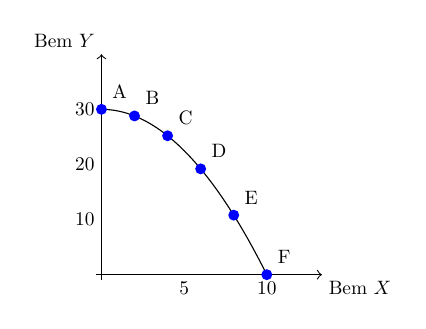
\begin{tikzpicture}[
					scale=0.7,
					every node/.style={scale=0.7},
					declare function = {fpp(\x) = 3 - (1/3) * \x^(2);}
					]

					\draw[->] (-0.1,0) -- (4,0) node[below right] {Bem $X$};
					\draw[->] (0,-0.1) -- (0,4) node[above left] {Bem $Y$};

					\draw[smooth,domain=0:3,variable=\x] plot (\x,{fpp(\x)});

					\draw (0,{fpp(0)}) node[blue,circle,fill,inner sep=2pt,label=above right:A]{};
					\draw (0.6,{fpp(0.6)}) node[blue,circle,fill,inner sep=2pt,label=above right:B]{};
					\draw (1.2,{fpp(1.2)}) node[blue,circle,fill,inner sep=2pt,label=above right:C]{};
					\draw (1.8,{fpp(1.8)}) node[blue,circle,fill,inner sep=2pt,label=above right:D]{};
					\draw (2.4,{fpp(2.4)}) node[blue,circle,fill,inner sep=2pt,label=above right:E]{};
					\draw (3,{fpp(3)}) node[blue,circle,fill,inner sep=2pt,label=above right:F]{};

					\draw (0,3) node[left] {30};
					\draw (0,2) node[left] {20};
					\draw (0,1) node[left] {10};

					\draw(1.5,0) node[below] {5};
					\draw(3,0) node[below] {10};

				\end{tikzpicture}
			\end{center}
		\end{column}
	\end{columns}
\end{frame}

\begin{frame}
	\frametitle{Custo relativo}
	$$CO_X = TMT_{Y,X}=-\frac{\Delta Y}{\Delta X}$$
	\begin{center}
		\begin{tabular}{cccc}
			Possibilidade de produ\c c\~ao & Bem $X$ & Bem $Y$ & $TMT_{Y,X}$ \\
			\hline\hline
			A & 0 & 30 & - \\
			B & 2 & 28 & 1 \\
			C & 4 & 24 & 2 \\
			D & 6 & 18 & 3 \\
			E & 8 & 10 & 4 \\
			F & 10 & 0 & 5 \\
			\hline \hline
		\end{tabular}
	\end{center}
\end{frame}

\begin{frame}
	\frametitle{Custo Relativo Crescente}
	\begin{center}
		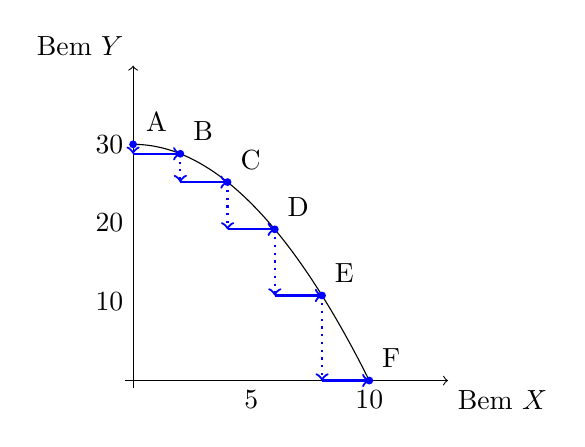
\begin{tikzpicture}[
			scale=1,
			every node/.style={scale=1},
			declare function = {fpp(\x) = 3 - (1/3) * \x^(2);}
			]

			\draw[->] (-0.1,0) -- (4,0) node[below right] {Bem $X$};
			\draw[->] (0,-0.1) -- (0,4) node[above left] {Bem $Y$};

			\draw[smooth,domain=0:3,variable=\x] plot (\x,{fpp(\x)});

			\draw (0,{fpp(0)}) node[blue,circle,fill,inner sep=1pt,label=above right:A]{};
			\draw (0.6,{fpp(0.6)}) node[blue,circle,fill,inner sep=1pt,label=above right:B]{};
			\draw (1.2,{fpp(1.2)}) node[blue,circle,fill,inner sep=1pt,label=above right:C]{};
			\draw (1.8,{fpp(1.8)}) node[blue,circle,fill,inner sep=1pt,label=above right:D]{};
			\draw (2.4,{fpp(2.4)}) node[blue,circle,fill,inner sep=1pt,label=above right:E]{};
			\draw (3,{fpp(3)}) node[blue,circle,fill,inner sep=1pt,label=above right:F]{};

			\draw (0,3) node[left] {30};
			\draw (0,2) node[left] {20};
			\draw (0,1) node[left] {10};

			\draw(1.5,0) node[below] {5};
			\draw(3,0) node[below] {10};

			\foreach \x in {0,...,4}
				{
				\draw[blue,thick,dotted,->] ({\x*0.6},{fpp((\x*0.6))}) -- ({\x*0.6},{fpp((\x*0.6+0.6))});
				\draw[blue,thick,->] ({\x*0.6},{fpp((\x*0.6+0.6))}) -- ({(\x*0.6+0.6)},{fpp((\x*0.6+0.6))});
				}	

		\end{tikzpicture}
	\end{center}

\end{frame}

\begin{frame}
	\frametitle{Custo Relativo - Derivada da FPP}
	\begin{columns}
		\begin{column}{0.47\textwidth}
			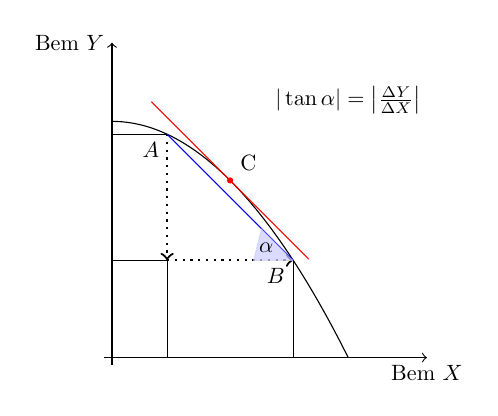
\begin{tikzpicture}[
			scale=1,
			every node/.style={scale=0.8},
			declare function = {fpp(\x) = 3 - (1/3) * \x^(2);},
			declare function = {tfpp(\x) = (15/4) - \x;}
			]
			\def\a{0.7}
			\def\b{2.3}
			\def\d{1.5}

			\draw[->] (-0.1,0) -- (4,0) node[below] {Bem $X$};
			\draw[->] (0,-0.1) -- (0,4) node[left] {Bem $Y$};

			\draw[smooth,domain=0:3,variable=\x] plot (\x,{fpp(\x)});

			\draw (3,3) node[above] {$|\tan \alpha|=\left|\frac{\Delta Y}{\Delta X}\right|$};

			\draw (0,{fpp(\a)}) -- (\a,{fpp(\a)}) node[below left] {$A$};
			\draw (0,{fpp(\b)}) -- (\a,{fpp(\b)});
			\draw[dotted,thick,->] (\a,{fpp(\a)}) -- (\a,{fpp(\b)});
			\draw[dotted,thick,->] (\a,{fpp(\b)}) -- (\b,{fpp(\b)})node[below left] {$B$};
			\draw (\a,{fpp(\b)}) -- (\a,0);
			\draw (\b,{fpp(\b)}) -- (\b,0);

			\draw[blue] (\a,{fpp(\a)}) -- (\b,{fpp(\b)});

			\draw[red,domain=0.5:2.5,variable=\x] plot (\x,{tfpp(\x)});
			\draw (\d,{fpp(\d)}) node[red,circle,fill,inner sep=1pt,label=above right:C]{};

			\draw[fill,blue!20,opacity=0.7] (\b,{fpp(\b)}) -- ({(\b-0.5)},{fpp(\b)}) -- ({\b-0.4},{fpp(\b)+0.4});
			\draw (\b-0.15,{fpp(\b)}) node[above left] {$\alpha$};

			\end{tikzpicture}
		\end{column}
		\begin{column}{0.47\textwidth}
			{\scriptsize
			\begin{itemize}
				\item $\frac{\Delta Y}{\Delta X}$ \'e a taxa de varia\c c\~ao m\'edia: qual a varia\c c\~ao em $Y$ por unidade de varia\c c\~ao em $X$...
				\item $\left|\frac{\Delta Y}{\Delta X}\right|$ \'e o custo relativo de uma unidade adicional de $X$
				\item $\left|\frac{\Delta Y}{\Delta X}\right|$ \'e o custo de oportunidade de uma unidade adicional de $X$
				\item $\frac{\Delta Y}{\Delta X}$ \'e o declive da recta tangente no ponto $C$ (Lagrange)... \'e a derivada \`a FPP nesse ponto
			\end{itemize}
			}
		\end{column}
	\end{columns}
\end{frame}

\begin{frame}
	\frametitle{Vantagens do Com\'ercio}
	Vamos admitir que podemos aceder a um mercado onde podemos transacionar $y$ unidades do bem $Y$ por $x$ unidades do bem $X$. O que temos ent\~ao \'e algo similar ao que t\'inhamos na aula anterior, termos de troca constantes, mas a nossa FPP n\~ao mudou.
	\begin{center}
		\begin{tikzpicture}[
				scale=1,
				every node/.style={scale=0.8},
				declare function = {fpp(\x) = 3 - (1/3) * \x^(2);},
				declare function = {mkt1(\x) = 3 - 0.8*\x;},
				declare function = {mkt2(\x) = 4 - 0.8*\x;},
				declare function = {mkt3(\x) = 3.5 - 0.8*\x;}
				]

				\draw[->] (-0.1,0) -- (5.2,0) node[below] {Bem $X$};
				\draw[->] (0,-0.1) -- (0,5) node[left] {Bem $Y$};

				\draw[smooth,domain=0:3,variable=\x] plot (\x,{fpp(\x)});
				\draw (0,{fpp(0)}) node[left] {$Y_0$};
				\draw (3,{fpp(3)})node[below] {$X_0$};
				
				\only<2>{
					\draw[red,domain=0:(3/0.8),variable=\x] plot (\x,{mkt1(\x)});
				}

				\only<3>{
					\draw[red,dashed,domain=0:2.45,variable=\x] plot (\x,{mkt1(\x)});
					\draw[red,domain=2.45:(3/0.8),variable=\x] plot (\x,{mkt1(\x)});
				}

				\only<4>{
					\draw[red,domain=0:(4/0.8),variable=\x] plot (\x,{mkt2(\x)});
				}

				\only<5>{
					\draw[red,domain=0:(3.5/0.8),variable=\x] plot (\x,{mkt3(\x)});
				}


		\end{tikzpicture}
	\end{center}
\end{frame}

\begin{frame}
	\frametitle{Vantagens do Com\'ercio}
	\begin{columns}
		\begin{column}{0.47\textwidth}
			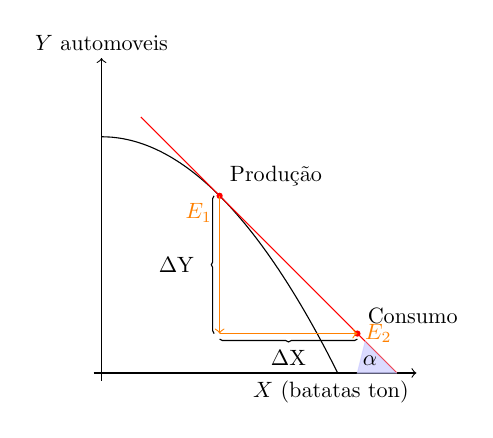
\begin{tikzpicture}[
			scale=1,
			every node/.style={scale=0.8},
			declare function = {fpp(\x) = 3 - (1/3) * \x^(2);},
			declare function = {tfpp(\x) = (15/4) - \x;}
			]

			\def\d{1.5}
			\def\e{3.25}

			\draw[->] (-0.1,0) -- (4,0) node[below left] {$X$ (batatas ton)};
			\draw[->] (0,-0.1) -- (0,4) node[above] {$Y$ automoveis};

			\draw[smooth,domain=0:3,variable=\x] plot (\x,{fpp(\x)});

			\draw[red,domain=0.5:(15/4),variable=\x] plot (\x,{tfpp(\x)});
			\draw (\d,{fpp(\d)}) node[red,circle,fill,inner sep=1pt,label=above right:Produ\c c\~ao]{};
			\draw (\e,{tfpp(\e)}) node[red,circle,fill,inner sep=1pt,label=above right:Consumo]{};

			\draw[orange,->] (\d,{fpp(\d)}) node[below left] {$E_1$} -- (\d,{tfpp(\e)});
			\draw[orange,->] (\d,{tfpp(\e)}) -- (\e,{tfpp(\e)}) node[right] {$E_2$};

			\draw[fill,blue!20,opacity=0.7] ({(15/4)},{tfpp((15/4))}) -- ({(15/4)-0.5},{tfpp((15/4))}) -- ({(15/4)-0.4},{tfpp((15/4))+0.4});
			\draw ({(15/4)-0.15},{tfpp((15/4))}) node[above left] {$\alpha$};

			\draw [decorate,decoration={brace,amplitude=1pt},xshift=-2pt,yshift=0pt] (\d,{tfpp(\e)}) -- (\d,{tfpp(\d)}) node [black,midway,xshift=-0.6cm] {$\Delta$Y};
			\draw [decorate,decoration={brace,mirror,amplitude=1pt},xshift=0pt,yshift=-2pt] (\d,{tfpp(\e)}) -- (\e,{tfpp(\e)}) node [black,midway,yshift=-0.3cm] {$\Delta$X};

			\end{tikzpicture}
			$\Delta Y$: Exporta\c c\~ao\\
			$\Delta X$: Importa\c c\~ao
		\end{column}
		\begin{column}{0.47\textwidth}
			{\scriptsize
			\begin{itemize}
				\item 1 autom\'ovel vende-se internacionalmente por $p_y=\textup{\euro}8,000$
				\item 1 ton de batatas vende-se internacionalmente por $p_x=\textup{\euro}1,000$
				\item Termos de troca: 1 autom\'ovel troca-se por 8 ton de batata $\frac{p_x}{p_y}=\frac{1}{8}$
				\item A fronteira de possibilidades de consumo ter\'a declive $\frac{1}{8}$ a partir do ponto de produ\c c\~ao $E_1$.
				\item Se o consumo for em $E_2$, esta economia exporta automoveis para importar batatas e verifica-se que:$$\Delta Y p_y + \Delta X p_x = 0$$
			\end{itemize}
			}
		\end{column}
	\end{columns}
\end{frame}

\begin{frame}
	\frametitle{Vantagens do Com\'ercio}
	\begin{columns}
		\begin{column}{0.47\textwidth}
			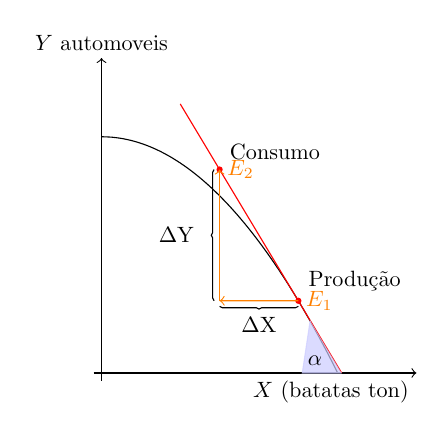
\begin{tikzpicture}[
			scale=1,
			every node/.style={scale=0.8},
			declare function = {fpp(\x) = 3 - (1/3) * \x^(2);},
			declare function = {tfpp(\x) = (61/12) - (5/3)*\x;}
			]

			\def\d{2.5}
			\def\e{1.5}

			\draw[->] (-0.1,0) -- (4,0) node[below left] {$X$ (batatas ton)};
			\draw[->] (0,-0.1) -- (0,4) node[above] {$Y$ automoveis};

			\draw[smooth,domain=0:3,variable=\x] plot (\x,{fpp(\x)});
			\draw[red,domain=1:3.05,variable=\x] plot (\x,{tfpp(\x)});

			\draw (\d,{fpp(\d)}) node[red,circle,fill,inner sep=1pt,label=above right:Produ\c c\~ao]{};
			\draw (\e,{tfpp(\e)}) node[red,circle,fill,inner sep=1pt,label=above right:Consumo]{};

			\draw[orange,->] (\d,{fpp(\d)}) node[right] {$E_1$} -- (\e,{tfpp(\d)});
			\draw[orange,->] (\e,{tfpp(\d)}) -- (\e,{tfpp(\e)}) node[right] {$E_2$};

			\draw[fill,blue!20,opacity=0.7] (3.05,{tfpp((3.05))}) -- ({3.05-0.5},{tfpp(3.05)}) -- ({3.05-0.4},{tfpp(3.05-0.4)});
			\draw ({3-0.1},{tfpp(3.05)}) node[above left] {$\alpha$};

			\draw [decorate,decoration={brace,amplitude=1pt},xshift=-2pt,yshift=0pt] (\e,{tfpp(\d)}) -- (\e,{tfpp(\e)}) node [black,midway,xshift=-0.6cm] {$\Delta$Y};
			\draw [decorate,decoration={brace,mirror,amplitude=1pt},xshift=0pt,yshift=-2pt] (\e,{tfpp(\d)}) -- (\d,{tfpp(\d)}) node [black,midway,yshift=-0.3cm] {$\Delta$X};

			\end{tikzpicture}
			$\Delta Y$: Importa\c c\~ao\\
			$\Delta X$: Exporta\c c\~ao
		\end{column}
		\begin{column}{0.47\textwidth}
			{\scriptsize
			\begin{itemize}
				\item Uma unidade de $Y$ vende-se internacionalmente por $p_y$
				\item Uma unidade de $X$ vende-se internacionalmente por $p_x$
				\item Termos de troca: 1 unidade de $X$ troca-se por $\frac{p_x}{p_y}$ unidades de $Y$
				\item O ponto de produ\c c\~ao \'e $E_1$, comum \`a FPP e a uma FPC de declive $\frac{p_x}{p_y}=|\tan \alpha|$
			\end{itemize}
			}
		\end{column}
	\end{columns}
\end{frame}

\begin{frame}
	\frametitle{Vantagens do Com\'ercio}
	\begin{columns}
		\begin{column}{0.47\textwidth}
			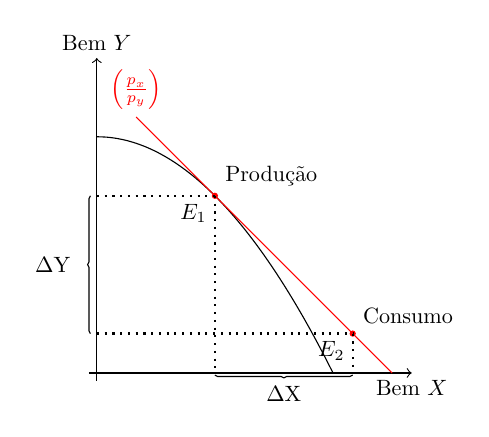
\begin{tikzpicture}[
			scale=1,
			every node/.style={scale=0.8},
			declare function = {fpp(\x) = 3 - (1/3) * \x^(2);},
			declare function = {tfpp(\x) = (15/4) - \x;}
			]

			\def\d{1.5}
			\def\e{3.25}

			\draw[->] (-0.1,0) -- (4,0) node[below] {Bem $X$};
			\draw[->] (0,-0.1) -- (0,4) node[above] {Bem $Y$};

			\draw[smooth,domain=0:3,variable=\x] plot (\x,{fpp(\x)});

			\draw[red,domain=0.5:(15/4),variable=\x] plot (\x,{tfpp(\x)});
			\draw[red] ({1/2},{tfpp(1/2)}) node [above] {$\left(\frac{p_x}{p_y}\right)$};
			\draw (\d,{fpp(\d)}) node[red,circle,fill,inner sep=1pt,label=above right:Produ\c c\~ao]{};
			\draw (\e,{tfpp(\e)}) node[red,circle,fill,inner sep=1pt,label=above right:Consumo]{};

			\draw[dotted, thick] (\d,{tfpp(\d)}) node[below left] {$E_1$} -- (\d,0);
			\draw[dotted, thick] (\e,{tfpp(\e)}) -- (\e,0);
			\draw[dotted, thick] (0,{tfpp(\e)}) -- (\e,{tfpp(\e)}) node[below left] {$E_2$};
			\draw[dotted, thick] (0,{tfpp(\d)}) -- (\d,{tfpp(\d)});

			\draw [decorate,decoration={brace,amplitude=1pt},xshift=-45pt,yshift=0pt] (\d,{tfpp(\e)}) -- (\d,{tfpp(\d)}) node [black,midway,xshift=-0.6cm] {$\Delta$Y};
			\draw [decorate,decoration={brace,mirror,amplitude=1pt},xshift=0pt,yshift=-15pt] (\d,{tfpp(\e)}) -- (\e,{tfpp(\e)}) node [black,midway,yshift=-0.3cm] {$\Delta$X};

			\end{tikzpicture}
		\end{column}
		\begin{column}{0.47\textwidth}
			{\scriptsize
			\begin{itemize}
				\item Termos de Troca no mercado: $\frac{p_x}{p_y}$
				\item Em $E_2$ verifica-se que: $$\Delta Y p_y + \Delta X p_x = 0$$
				\item Logo: $$\left|\frac{\Delta Y}{\Delta X}\right| =\frac{p_x}{p_y}$$
			\end{itemize}
			}
		\end{column}
	\end{columns}
\end{frame}

\begin{frame}
	\frametitle{Crescimento Econ\'omico}
	\begin{columns}
		\begin{column}{0.47\textwidth}
			\begin{tikzpicture}[
			scale=1,
			every node/.style={scale=0.8},
			declare function = {fpp1(\x) = 3 - (1/3) * \x^(2);},
			declare function = {fpp2(\x) = 3.5 - (1/3.5) * \x^(2);}
			]

				\draw[->] (-0.1,0) -- (4,0) node[below] {Bem $X$};
				\draw[->] (0,-0.1) -- (0,4) node[above] {Bem $Y$};

				\draw[smooth,domain=0:3,variable=\x] plot (\x,{fpp1(\x)});
				\draw[smooth,domain=0:3.5,variable=\x] plot (\x,{fpp2(\x)});

				\draw[->] (2,{fpp1(2)}) -- (2.4,{fpp2{2.4}});

			\end{tikzpicture}
		\end{column}
		\begin{column}{0.47\textwidth}
			\begin{tikzpicture}[
			scale=1,
			every node/.style={scale=0.8},
			declare function = {fpp1(\x) = 3 - (1/3) * \x^(2);},
			declare function = {fpp2(\x) = 3 - (1/3) * \x^(1.75);}
			]

				\draw[->] (-0.1,0) -- (4,0) node[below] {Bem $X$};
				\draw[->] (0,-0.1) -- (0,4) node[above] {Bem $Y$};

				\draw[smooth,domain=0:3,variable=\x] plot (\x,{fpp1(\x)});
				\draw[smooth,domain=0:3.5,variable=\x] plot (\x,{fpp2(\x)});

				\draw[->] (2.85,{fpp1(2.85)}) -- (3.3,{fpp2(3.3)});

			\end{tikzpicture}
		\end{column}
	\end{columns}
\end{frame}